\subsection{Introducción}
 Para poder aplicar el algoritmo propuesto con las instancias obtenidas de la TSPLIB, se desarrolló un programa utilizando el lenguaje de programación JAVA que permita almacenar datos en diferentes formatos (XML, JSON,TSPLIB).\\
 \hspace*{1cm}Otro propósito de este programa es que sea de código abierto con el fin de que otras personas puedan continuar con la investigación o utilizarlo como referencia para otros proyectos. Una vez que se explique la composición del software y la forma en la que se utiliza en el siguiente capítulo se procederá al desarrollo de los experimentos.\\
 
\subsection{Componentes} 
En la figura \ref {fig:Software_1} se muestra la ventana principal del programa que está compuesto por:
    \begin{enumerate}[label=\Alph*.-]
    \item Una barra de herramientas
    \item 3 pestañas cuyo contenido se explicará a continuación
    \item La pantalla principal que muestra un problema de TSP
    \end{enumerate}
\hspace*{1cm}Como se observa en la figura \ref {fig:Software_1} la ventana muestra la posición de los puntos del problema y las rutas que éste recorrió de principio a fin; también se muestran los cuadrantes que se trazaron para realizar el cálculo así como el orden de puntos en que se fue recorriendo.\\ 
     \begin{figure}[hbtp]
        \centering
            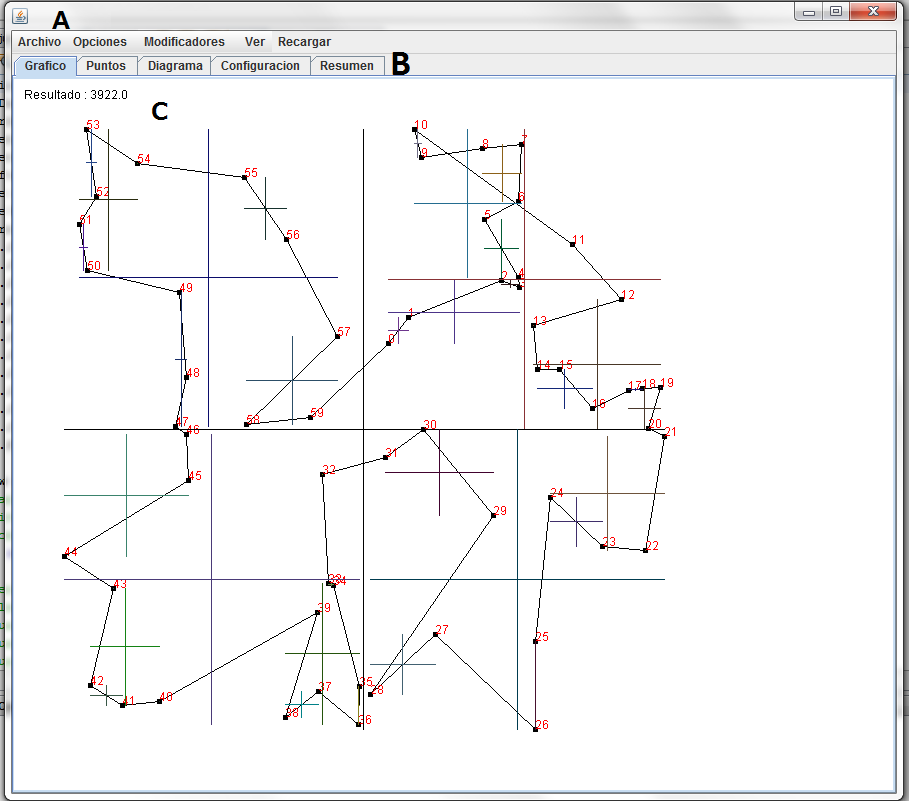
\includegraphics[width=1\textwidth]{Software/Imagenes/Software_1.png}
            \caption{Descripción de la ventana principal del software.}
            \label{fig:Software_1}
    \end{figure}

\hspace*{1cm}En la figura \ref {fig:Software_2} se muestran las coordenadas de los puntos del problema junto con el resultado mostrado en la figura \ref {fig:Software_1}.\\
     \begin{figure}[hbtp]
        \centering
            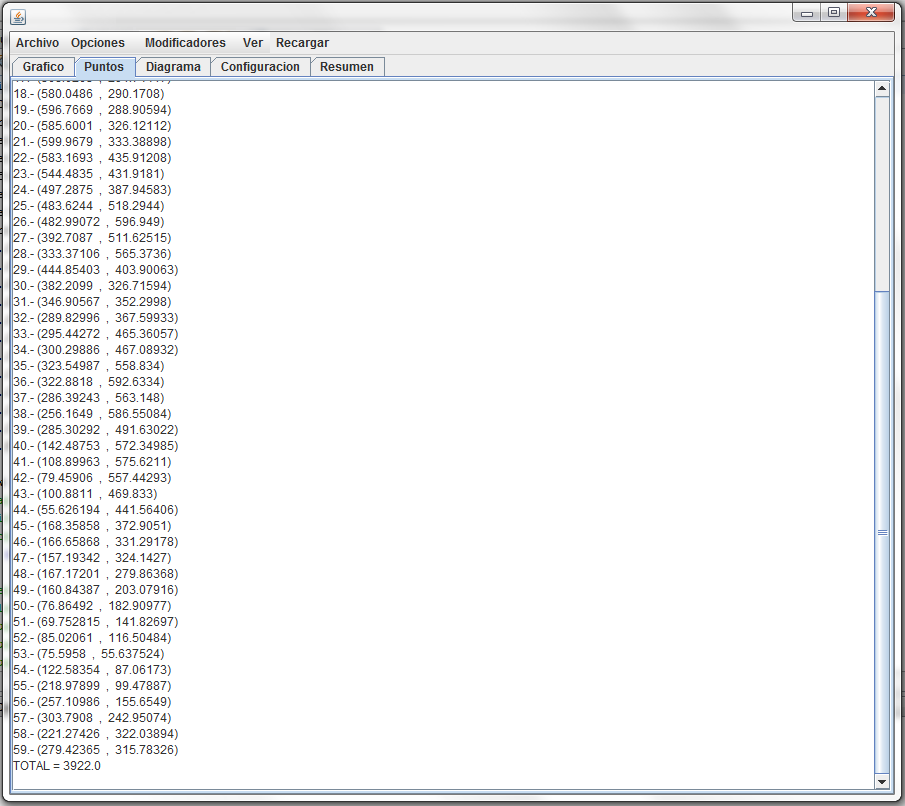
\includegraphics[width=0.4\textwidth]{Software/Imagenes/Software_2.png}
            \caption{Coordenadas de los puntos del problema.}
            \label{fig:Software_2}
    \end{figure}
    
\hspace*{1cm}En la figura \ref {fig:Software_3} se muestra la gráfica de los resultados obtenidos en el problema utilizando diferentes metaheurísticas. En este ejemplo se aplicó únicamente el algoritmo de recocido simulado.\\
     \begin{figure}[hbtp]
        \centering
            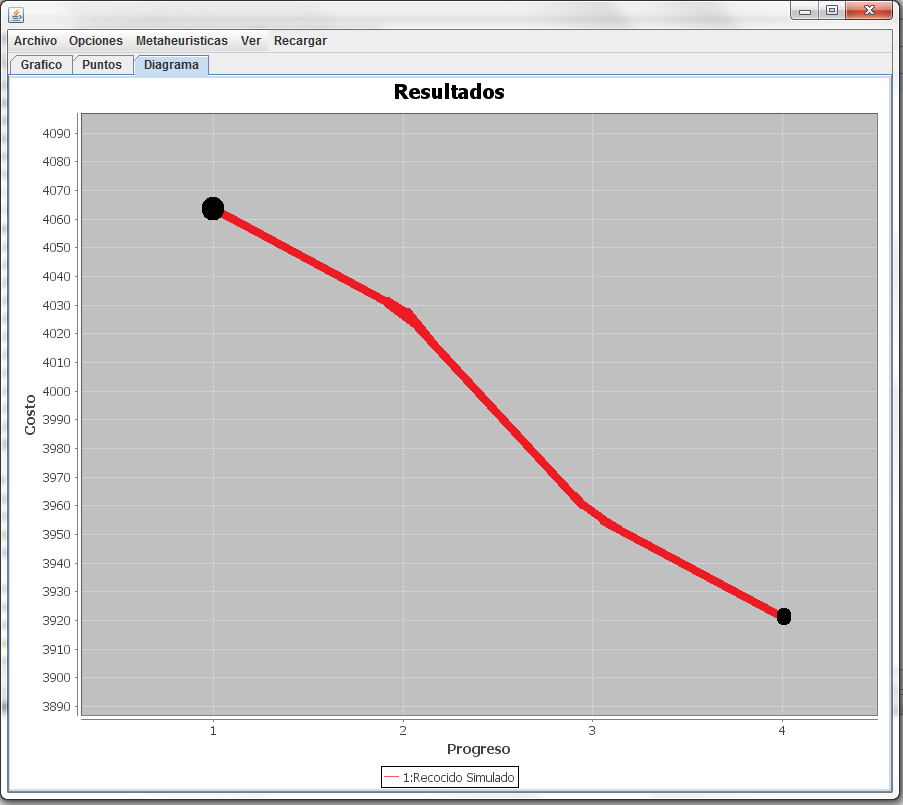
\includegraphics[width=0.4\textwidth]{Software/Imagenes/Software_3.png}
            \caption{Gráfica de los resultados del problema.}
            \label{fig:Software_3}
    \end{figure}
  
\hspace*{1cm}En la figura \ref {fig:Software_9} se muestra la ventana de configuraciones que se puede realizar para cada metaheurística, como la cantidad de ciclos que se puede hacer, el tamaño de los genes, factor de temperatura para el proceso de recocido simulado, etc. El uso de estas variables se explicarán en el siguiente capítulo.\\
     \begin{figure}[hbtp]
        \centering
            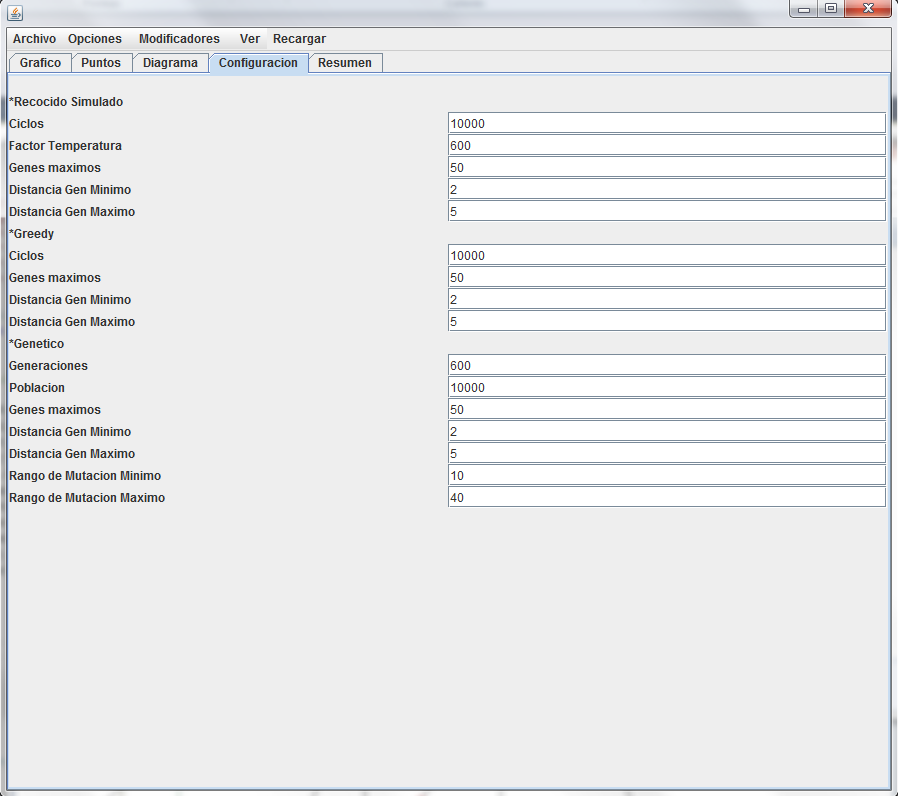
\includegraphics[width=0.6\textwidth]{Software/Imagenes/Software_9.png}
            \caption{Ventana de configuración.}
            \label{fig:Software_9}
    \end{figure}
    
\hspace*{1cm}En la figura \ref {fig:Software_10} se muestra una pantalla que despliega la cantidad de tiempo que tarda el algoritmo cada vez que se ejecuta un problema.\\
     \begin{figure}[hbtp]
        \centering
            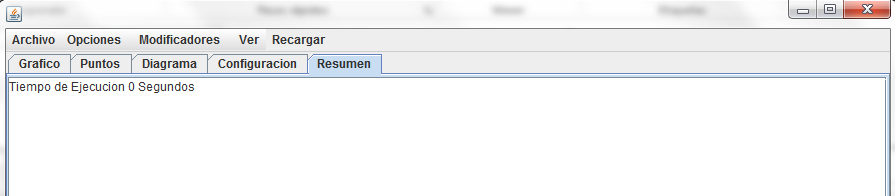
\includegraphics[width=0.7\textwidth]{Software/Imagenes/Software_10.png}
            \caption{Ventana de resultados.}
            \label{fig:Software_10}
    \end{figure}
    
\hspace*{1cm}En la figura \ref {fig:Software_4} se puede observar el menú de Archivo de la barra de herramientas, que tiene las siguientes opciones:

\begin{enumerate}[label=\Alph*.-]
\item \textbf{Guardar:} Permite guardar las coordenadas para poder usarse en experimentos futuros en un archivo .TSP.
\item \textbf{Abrir:} Abre un documento .TSPLIB o .TXT y carga sus coordenadas en el programa, una vez que se carguen los datos el problema se resolverá automáticamente.
\item \textbf{Abrir sin resolver:}Lo mismo que el botón anterior, solo que no resuelve el problema de forma automática.
\item \textbf{Abrir Prueba:} Permite abrir un archivo XML ó JSON y cargar un problema con sus respectivos resultados. Estos problemas se consiguen a través de los siguientes botones.
\item \textbf{Guardar (XML):} Permite guardar un problema con todos los resultados obtenidos en un archivo XML.
\item \textbf{Guardar (JSON):} Lo mismo que el anterior, pero lo guarda en formato JSON.
\item \textbf{Realizar Experimento:} Este será la función que se usará para realizar las actividades del siguiente capítulo, permite realizar de manera consecutiva una serie de ejecuciones del mismo listado de puntos que se encuentra cargados, guardando los resultados de forma física con el archivo .JSON de cada resultado y su gráfica correspondiente. Por ejemplo si se seleccionan 30 ejecuciones devolverá 30 archivos .json y 30 gráficas de cada uno.
\end{enumerate}

     \begin{figure}[hbtp]
        \centering
            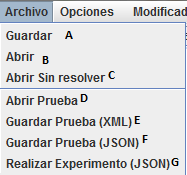
\includegraphics{Software/Imagenes/Software_4.png}
            \caption{Barra de herramientas, Archivo.}
            \label{fig:Software_4}
    \end{figure}
    
\hspace*{1cm}En la figura \ref {fig:Software_5} se muestra el menú de Opciones, la cual contiene funciones de diversos propósitos:
\begin{enumerate}[label=\Alph*.-]
\item  \textbf{Aleatorio:} Permite generar una serie de coordenadas al azar y que resolverá de manera automática, el propósito original de esta función fue la de probar el algoritmo de búsqueda por cuadrantes conforme se fue desarrollando.
\item  \textbf{Borrar resumen:} Permite limpiar la pantalla de la ventana de resumen de la figura \ref {fig:Software_10}.
\end{enumerate}
     \begin{figure}[hbtp]
        \centering
            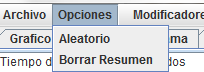
\includegraphics{Software/Imagenes/Software_5.png}
            \caption{Barra de herramientas, Opciones.}
            \label{fig:Software_5}
    \end{figure}

\hspace*{1cm}En la figura \ref {fig:Software_6} se puede observar el menú de modificadores que se encarga de aplicar las perturbaciones de la solución base; éstas se harán al final de la ejecución del método de cuadrantes (si se marcó como seleccionado el método de cuadrantes) con el fin de optimizar la solución base, los algoritmos que se pueden seleccionar son:
    
\begin{enumerate}[label=\Alph*.-]
\item Cuadrantes 
\item Búsqueda Exhaustiva
\item Recocido Simulado
\item Búsqueda Greedy
\item Algoritmo Genético
\end{enumerate}

     \begin{figure}[hbtp]
        \centering
            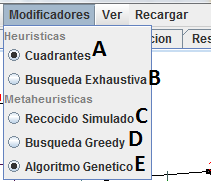
\includegraphics[width=0.3\textwidth]{Software/Imagenes/Software_6.png}
            \caption{Barra de herramientas, Modificadores.}
            \label{fig:Software_6}
    \end{figure}
    
\hspace*{1cm}En la figura \ref {fig:Software_7} se puede observar el menú de Ver, que permite dibujar el diagrama de la figura \ref {fig:Software_1} de acuerdo a los elementos que aparecen en el listado:

\begin{enumerate}[label=\Alph*.-]
\item \textbf{Ruta:} Las líneas que muestra el recorrido de punto a punto.
\item \textbf{Puntos:}Los nodos que indican la ubicación exacta de cada punto.
\item \textbf{Lineas:} Las divisiones de colores que los cuadrantes de acuerdo al método de cuadrantes.
\item \textbf{Números:} El orden de los puntos que recorrió la ruta de principio a fin.
\item \textbf{Final:} La última ruta que se recorre del último punto hacia el punto de inicio.
\end{enumerate}

     \begin{figure}[hbtp]
        \centering
            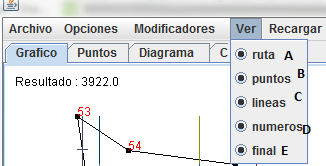
\includegraphics[width=0.7\textwidth]{Software/Imagenes/Software_7.png}
            \caption{Barra de herramientas, Ver.}
            \label{fig:Software_7}
    \end{figure}
    
\hspace*{1cm}En la figura \ref {fig:Software_8} se puede observar la opción de Recargar que permite volver a generar el problema; la utilidad de esta función es la de reutilizar el mismo problema usando los diferentes métodos de la figura \ref {fig:Software_6} o bien, esperar obtener resultados diferentes.\\

     \begin{figure}[hbtp]
        \centering
            
\includegraphics{Software/Imagenes/Software_8.png}
            \caption{Barra de herramientas, Recargar.}
            \label{fig:Software_8}
    \end{figure}
    
\subsection{Uso del software}
Ya conociendo los componentes que conforman el programa se procederá a explicar la manera en que se usará para los experimentos.\\
\hspace*{1cm}Al iniciar el programa se mostrará una ventana parecida a la de la figura \ref {fig:Software_1} donde se muestra un problema formado por un conjunto de puntos al azar ya resuelto, sin embargo para esta ocasión se usará un archivo .TSP como prueba. Primero se usará la opción de Abrir sin resolver como se muestra en la figura \ref {fig:Software_Uso_1}.
     \begin{figure}[hbtp]
        \centering
            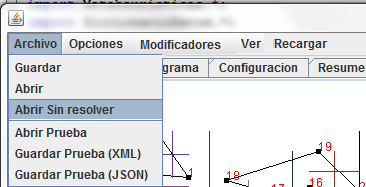
\includegraphics[width=0.5\textwidth]{Software/Imagenes/Software_Uso_1.png}
            \caption{Abrir sin resolver.}
            \label{fig:Software_Uso_1}
    \end{figure}
    
\hspace*{1cm}Para este ejemplo se usará el archivo 'ch150.tsp' como se muestra en la figura \ref {fig:Software_Uso_2}, la mejor ruta conocida para este problema es de 6528 unidades. 
     \begin{figure}[hbtp]
        \centering
            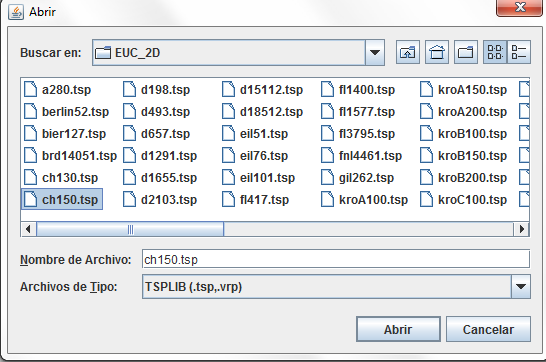
\includegraphics[width=0.55\textwidth]{Software/Imagenes/Software_Uso_2.png}
            \caption{Archivo .TSP.}
            \label{fig:Software_Uso_2}
    \end{figure}
    
\hspace*{1cm}En la figura \ref {fig:Software_Uso_3} se puede apreciar que los puntos se encuentran desordenados, por tanto genera una ruta de lo más ineficiente con un costo de 52890 unidades ya que uno los puntos en el mismo orden que los va leyendo.\\

    \begin{figure}[hbtp]
        \centering
            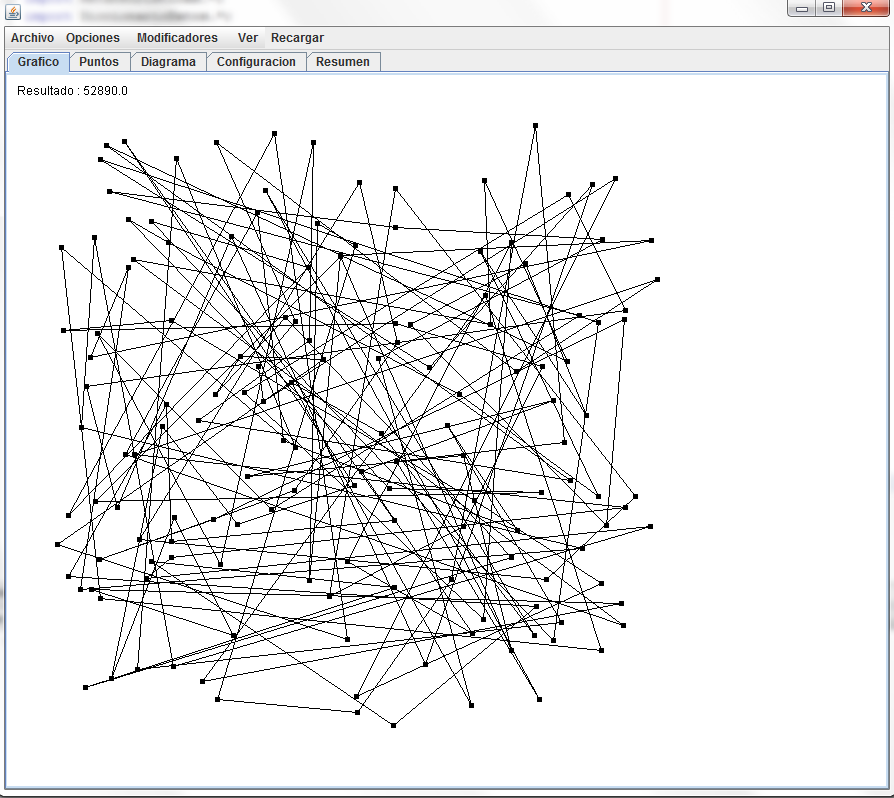
\includegraphics[width=0.9\textwidth]{Software/Imagenes/Software_Uso_3.png}
            \caption{Archivo sin resolver.}
            \label{fig:Software_Uso_3}
    \end{figure}

\clearpage \newpage

\hspace*{1cm}Sin embargo si se aplica la opción de recargar se aplicará las fórmulas que se tienen seleccionadas, en este caso solo se aplicará el método de cuadrantes, tal como se muestra en la figura \ref {fig:Software_Uso_4}. Los puntos siguen siendo los mismos pero el trazado de rutas está ordenado de acuerdo dicho método trayendo un costo de 8579 unidades, siendo menos de una sexta parte del costo de la figura \ref {fig:Software_Uso_3}.\\

    \begin{figure}[hbtp]
        \centering
            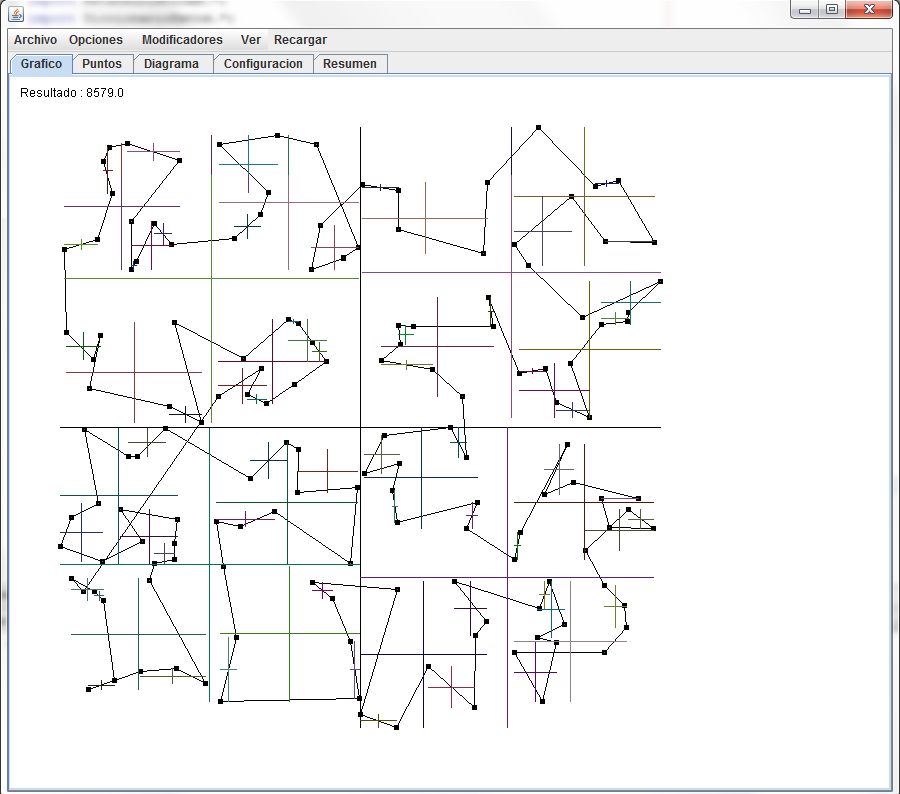
\includegraphics[width=0.9\textwidth]{Software/Imagenes/Software_Uso_4.png}
            \caption{Problema resuelto con el método de cuadrantes.}
            \label{fig:Software_Uso_4}
    \end{figure}
\clearpage \newpage

\hspace*{1cm}En la figura \ref {fig:Software_Uso_5} se volvió a recargar el mismo problema pero esta vez usando el método de búsqueda exhaustiva la cual trae un valor de 8252 unidades, un valor ligeramente menor al anterior con 327 unidades de diferencia.\\

    \begin{figure}[hbtp]
        \centering
            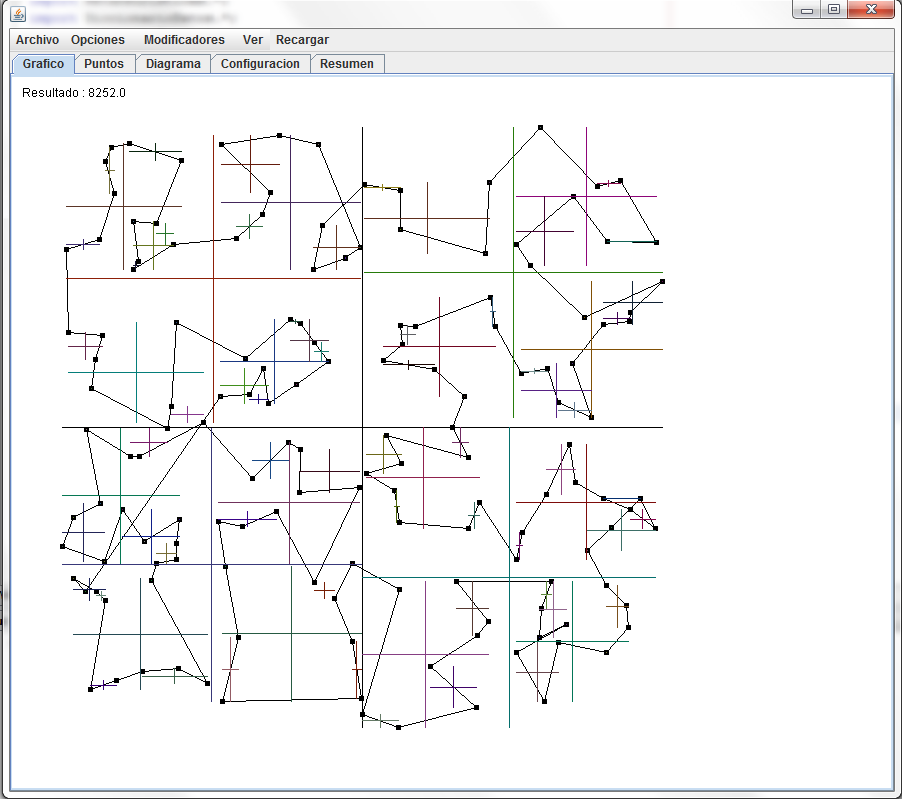
\includegraphics[width=0.9\textwidth]{Software/Imagenes/Software_Uso_5.png}
            \caption{Problema resuelto con el método de cuadrantes y la búsqueda exhaustiva en el orden correspondiente.}
            \label{fig:Software_Uso_5}
    \end{figure}
\clearpage \newpage

\hspace*{1cm}En la figura \ref {fig:Software_Uso_6} se volvió a recargar el mismo problema pero esta vez marcando también el método de recocido simulado con un resultado de 8179 unidades, una mejora de la figura \ref {fig:Software_Uso_5} con 73 unidades de diferencia.\\

    \begin{figure}[hbtp]
        \centering
            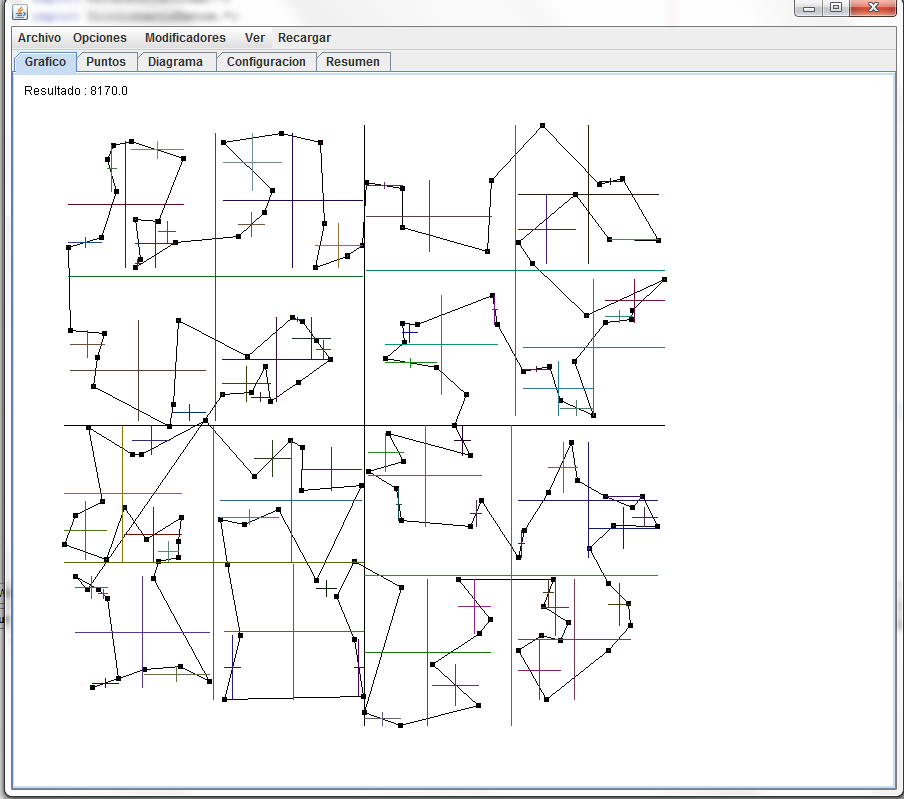
\includegraphics[width=0.9\textwidth]{Software/Imagenes/Software_Uso_6.png}
            \caption{Problema resuelto con el método de cuadrantes, recocido simulado y búsqueda exhaustiva en el orden correspondiente.}
            \label{fig:Software_Uso_6}
    \end{figure}
\clearpage \newpage

\hspace*{1cm}En la figura \ref {fig:Software_Uso_7} se puede mostrar la gráfica de la forma en que fue mejorando la solución obtenida por el programa. El método de Búsqueda exhaustiva siempre se ejecutará al final del proceso.\\

    \begin{figure}[hbtp]
        \centering
            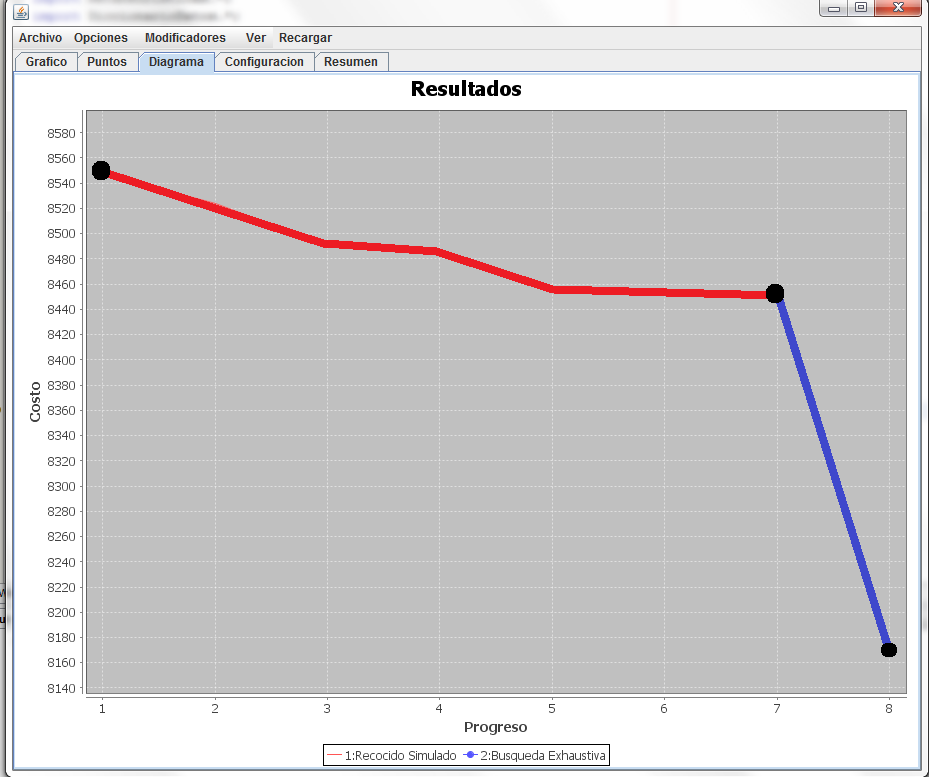
\includegraphics[width=0.9\textwidth]{Software/Imagenes/Software_Uso_7.png}
            \caption{Gráfica que muestra los resultados.}
            \label{fig:Software_Uso_7}
    \end{figure}
\clearpage \newpage

\hspace*{1cm}Por último, aplicando el algoritmo genético en la figura \ref {fig:Software_Uso_8} con el fin de obtener el mejor resultado posible, deja un costo de 7342 unidades con una notable diferencia de 837 unidades.\\

    \begin{figure}[hbtp]
        \centering
            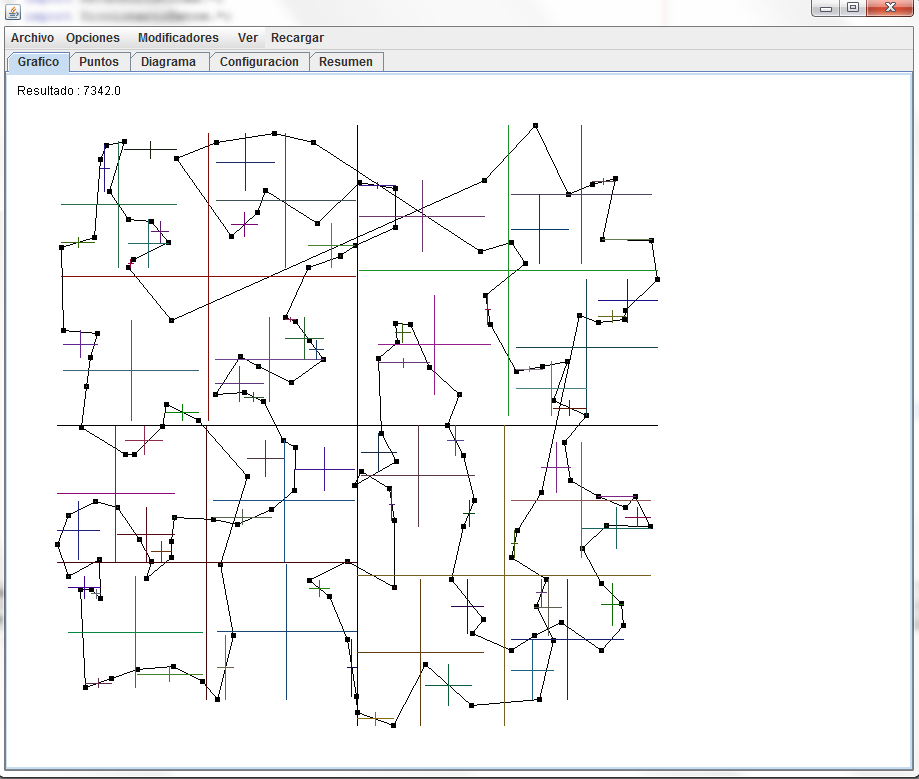
\includegraphics[width=0.9\textwidth]{Software/Imagenes/Software_Uso_8.png}
            \caption{Problema resuelto usando todas las metaheurísticas.}
            \label{fig:Software_Uso_8}
    \end{figure}
\clearpage \newpage

\hspace*{1cm}En la figura \ref {fig:Software_Uso_9}, se puede observar la gráfica con el resultado de la figura \ref {fig:Software_Uso_8} el cual muestra un resultado favorable en la línea que representa el algoritmo genético, debido a su simplicidad el método de búsqueda exhaustiva se aplica al final de las demás metahuerísticas.\\

    \begin{figure}[hbtp]
        \centering
            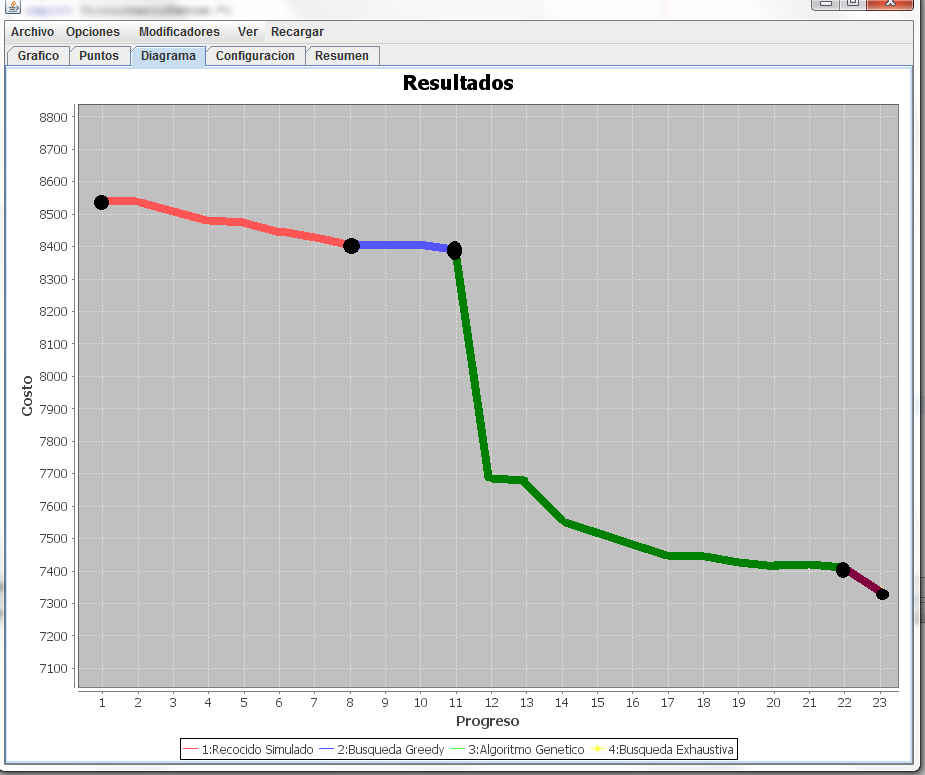
\includegraphics[width=0.9\textwidth]{Software/Imagenes/Software_Uso_9.png}
            \caption{Gráfica que muestra el progreso después de aplicar todas las metahuerísticas.}
            \label{fig:Software_Uso_9}
    \end{figure}  
\clearpage \newpage

\hspace*{1cm}Para finalizar si se desea mostrar el problema resuelto se puede guardar por medio de un archivo .XML o un .JSON descritos en la figura \ref {fig:Software_4}. En la figura \ref {fig:Software_Uso_10} se eligió en formato .JSON.\\
    \begin{figure}[hbtp]
        \centering
            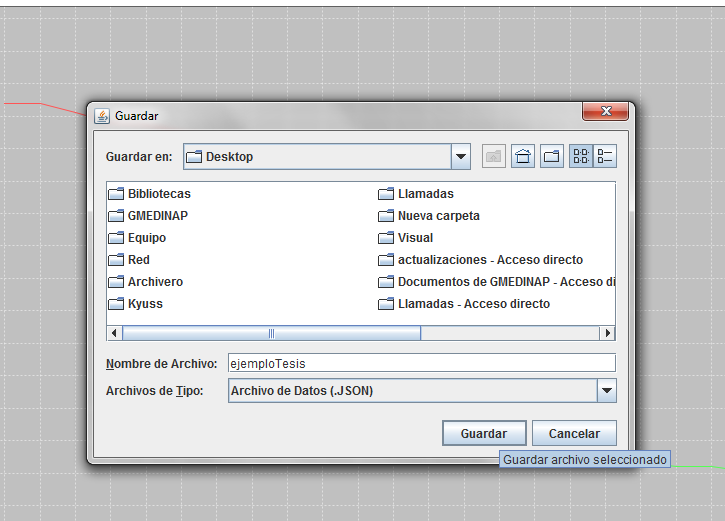
\includegraphics[width=0.5\textwidth]{Software/Imagenes/Software_Uso_10.png}
            \caption{Problema solucionado guardado en un JSON.}
            \label{fig:Software_Uso_10}
    \end{figure}

\subsection{Comentarios finales}
La ayuda de este programa fue esencial para poder realizar los experimentos, ya que gracias a esta herramienta fue posible leer, interpretar y almacenar los resultados correspondientes.\\
\hspace*{1cm}Una de las ventajas de este programa es que sigue el mismo formato de las TSPLIB, por tanto puede utilizarse para otros proyectos futuros, sin embargo solo está limitado a resolver problemas que utilizan distancia euclidiana (EUC2D).\\